\chapter{Linguistic Model Applications: NLP Semantic Tasks} 
\label{chap:wsd}
\begin{abstractchap}
Word Sense Induction and Disambiguation (WSD/WSI) is an elementary semantic NLP task useful to build larger systems. In this chapter, we leverage the network presented in the previous chapter and propose an algorithm that takes into account the structure of our model. Based on the real-world property of the network, we induce senses by grouping words that share a similar sense. We then assign these senses to target words. We show that our method improves on similar network-based methods.
\end{abstractchap}

\minitoc
\section{Word Sense Induction and Disambiguation}
\subsection{Introduction}
\label{chap5:intro}
In this chapter we employ the model introduced before to propose a solution to both Word Sense Disambiguation (WSD) and Induction  (WSI) tasks. We begin by giving a description and a succinct state of the art for both tasks. Specifically, we identify what type of language network (from those defined in Section\ref{sec:ling_networks}) is used and how.
%from a linguistic-network point of view.
We then present the characteristics of our proposed method. Finally we describe and discuss the obtained results.

%\subsection{Linguistic Networks in WSD and WSI}
\subsection{Related Work}

Word sense disambiguation, or WSD, is the task of examining a word in different contexts (we refer to a word in a particular context as an instance)  and determining which is the sense being used in each one of the contexts analyzed. Usually a list of senses from where to chose the correct one is given as an input. When this list is not available, WSD then becomes a different, complementary task: word sense induction, or WSI. WSI also analyses  tokens of a target word context but before assigning a sense to each of its instances, it first generates a list of possible senses from where to select from. 

\paragraph{Word Sense Disambiguation}In the literature \cite{2007.Sinha.Mihalcea.Unsupervised,2007.Tsatsaronis.WSDwithSpreading,2007.Navigli.GraphConnectivity,2009.Agirre.PersonalizedPageRankWSD,2010.Klapaftis.WSD.WSD.HierarchicalGraphs,2010.Siberer.GraphCooccurrenceWSD,2014.Moro.Navigli.EntityLinking_WSD}, WSD 
%2004.Mihalcea.SemanticNetworkPageRank,  2008.Agirre.Multilingual
is usually solved using semantic networks (SN). Specifically, Wordnet and to some extent BabelNet or Wikipedia (considering an article as a single concept).

The general process used to solve WSD follows a two-step algorithm. Given an input text with a words to disambiguate, and their corresponding context, WSD systems accomplish the following:
\begin{enumerate}
\item Link target words (usually nouns, without stop-words and functional words) with their corresponding  sense (or synset in the case of Wordnet-like dictionaries) and extract their vertices and edges into a new, smaller SN. 
\item Apply a node ranking technique, usually a random walk based method, and select, for each ambiguous word in the input text,  its top ranking synset node as the correct sense.
\end{enumerate}


The cited methods differences boil down to three aspects. Firstly, the type of semantic relation implied by the edges of the network. Secondly, the function used to  assign a weight to each edge, as well as its meaning. On the other hand, a common characteristic of these approaches is that, as said before, they all rely on semantic networks and thus are constrained by the limitations of such resources, mainly their static content and human annotated nature. 


We find that the use of a lexical knowledge base, such as Wordnet, is pervasive in this task. Indeed, new resources, such as BabelNet, solves to some extent the fixed (no new senses are included automatically) nature of this type of resources by leveraging the ever-evolving knowledge of Wikipedia. 

\paragraph{Word Sense Induction}We believe that in order to solve WSD in a truly end-to-end unsupervised way, one would need to automatically find a list of senses for a word without the help of pre-built semantic networks. In that sense, researchers generally use lexical co-occurrence networks, or LCNs, and thus leverage the distributional hypothesis, to automatically discover senses for a given target word. Therefore, WSI graph-based methods \cite{2004.Veronis,2007.Klapaftis.UOY,2010.Navigli.InducingWordSenses.Triangles,2008.Klapaftis.WSIUsingCollocations,2011.DiMarco.Navigli.ClusteringWebSearch,2011.Jurgens.WSICommunityDetection} are tightly related to LCNs.
 
Given an input document with a set of target words, coupled with a set of contexts (a target word in a unique context is called an instance), the goal is to discover a list of senses for each target word and then assign each instance in the document with an automatically generated sense. The common four steps used are the following:

\begin{enumerate}
\item Build a LCN, assigning tokens as nodes and  establishing edges between them if they co-occur in a given context (usually if they both appear in the same sentence, paragraph or fixed window of words).
\item Determine the weights for each edge according to a frequency metric. 
\item Apply a graph clustering algorithm. Each cluster found will represent a sense of the polysemous target word.
\item Match target word instances with the clusters found (the senses) by using the word context. Specifically, assign a sense to each instance by looking at the tokens in the context. This step is actually the word sense disambiguation task. 
\end{enumerate}	

As with WSD, while  LCNs used are mostly the same among approaches, there are certain moving parts that make up the difference between WSI approaches. The most common differences that   arise are:

\begin{itemize}
\item The clustering algorithm to find senses in the LCN graph.
\item The technique used to match context words to clusters.
\item The weight used in the graph edges.
\end{itemize}


WSI, while being a more flexible approach (language and word-domain independent, does not require human-made knowledge bases), its results are tightly linked to the quality of the clustering algorithm used on the language network built. 
%

%\paragraph{State of the art discussion}\label{sec:survey_disc}


With respect to the networks' structure, we find that few approaches include syntactic attributes into their model. We believe that finding semantic similarities can be improved by adding syntactic information not only  while using dependency relations but also by leveraging the constituency tree of each word. Moreover, using syntactic data along with semantic and/or lexical co-occurrences takes us into the heterogeneous network domain which has not been addressed in most of the approaches covered.
Being able to design new similarity metrics that deal with different types of information opens new avenues of research in the semantic similarity domain. % Finally, concerning the algorithms employed, few approaches make direct use of the graph Laplacian representation. New similarities could be defined using the Laplacian as a starting point. 




\subsection{Approach}
	
%The cited works use a LCN as described before while other works such as \cite{2014.Tao.Qian.LexicalChainHypergraphWSI} represent the co-occurrence by means of a hypergraph schema. In short, a hypergraph structure is a graph generalization where an edge (called hyperedge) can link multiple vertices per edge and thus it is able to provide a more complete description of the interactions between several nodes.


Formally, the objective of WSD/WSI is the following: given a document $d$ with a set $T$ of  target words $tw \in T$ and the set $C$ with contexts for each target word $ct_{tw}$. 
Specifically, each paragraph represents the context  of a target word. A target word in a specific context is also called an instance.
% $tw$. %Each word $tw$ features several $ct$.
The goal is first to solve the WSI task, that is, automatically determine a list of senses for a given $tw$, and then assign one meaning from this list to each of its instances, the WSD task.
%
%As described before, WSI  is usually solved following four steps: (1) creation of a linguistic network, (2) determine the level of similarity between nodes within the network, (3) cluster nodes together, thus creating individual senses, and (4)  assign a cluster (sense) to each instance of a target word in the input document (this step amounts to WSD).


Our method follows is inspired on previous approaches from \cite{2004.Veronis} and \cite{2007.Klapaftis.UOY}. In Hyperlex,  the graph-based  method presented  in \cite{2004.Veronis}, the main intuition is that co-occurrence networks have small-world properties and thus it is possible to detect and isolate important heavily-connected nodes, call "hubs". These hubs, and their connected nodes represent a sense in itself. 

Hyperlex performs WSI and WSD using a weighted lexical co-occurrence network. The process is performed for each target word in the document. As a first step, they build a  graph by defining the vertices (the target word node is removed) as the tokens found in the  co-occurring  context of a target word. The edges link two words co-occurring together. Each edge is assigned a weight that decreases as the association frequency of the words increases. The second step consists on iteratively finding the hubs and removing them, along with their adjacent nodes, from the target word graph. Again, the intuition of the method is that these isolated hubs, and their adjacent words, represent a sense of the analyzed word. The third and final step carries out the disambiguation. A new graph is created by adding the target word to the co-occurrence graph. Zero-weighted edges are added between each hub and the target word. A minimum spanning tree is then calculated and the sense component found to have the closest set of nodes is chosen as the target word sense.

The second approach, \textit{UOY}, described in \cite{2007.Klapaftis.UOY},  relies itself on the small-world intuition presented  by Hyperlex to find hubs and its adjacent nodes to represent senses.   In short, these methods, as ours, exploit the real-world characteristics of linguistic networks by theorizing that there are certain few high-degree nodes (called hubs) that carry an important role in the network and therefore may represent, coupled with their neighbors, a sense for a given target word. Particularly, UOY considers bigrams and trigrams that co-occur in a paragraph as hyperedges. Under a frequent-itemset setting, they determine important hyperedges given their \textit{support} and their \textit{confidence}  values. Then, the clustering of words takes place by finding the hubs and considering them as sense carriers only if they satisfy a threshold mainly set upon their containing-hyperedge confidence value. Finally, once the senses are identified, each target word instance (represented by a context) is assigned to a sense according to the sum of confidences of the hyperedge appearing on said context. 

In our method, we generate a network for each $tw$ and consider that the high-degree nodes inside this network may represent a $tw$ sense. In Algorithm \ref{alg:wsd} we show the general flow of our approach.  We detail the steps taken alongside the corresponding line in the algorithm below. 

\paragraph{Creation of the linguistic network}
%In the previous sections we worked with the English Wikipedia as background corpus to build and model our proposed linguistic network. Given the large size of Wikipedia, and to iterate faster our experiments, we decided to change the corpus to one with a more manageable size.

%We use the Open American National Corpus (OANC) \cite{oanc} as background document collection to build a hypergraph network $G_H$ following our proposed model.  The OANC  includes texts from several domains and encompasses 11,406,155 words. We split the documents of the corpus in sentences, then we tokenize and parse them with Stanford's CoreNLP \cite{corenlp}. As described before, the dependency and constituency tree are used to build the hypergraph: words are depicted by nodes, and they may exist inside any of the three different types of hyperedges defined (sentence,  noun phrase or dependency contexts). If any  hyperedge is repeated through the corpus, we increment a counter and keep the number of apparitions instead of adding redundant columns to the hypergraph incidence matrix.

In order to find senses from the contexts of a target word, the first step in our procedure is to build a linguistic graph $G_H$ from a background corpus. As described in previous sections, the dependency and constituency trees are used to build the hypergraph: words are depicted by nodes, and they may exist inside any of the three different types of hyperedges defined (sentence,  noun phrase or dependency contexts). If any  hyperedge is repeated through the corpus, we increment a counter and keep the number of apparitions instead of adding redundant columns to the hypergraph incidence matrix.

At each step, that is, for each $tw$ in the test input document, we extract a subgraph $G_{tw}$ from $G_H$ that contains all the words that appear together with $tw$ (line 2), whether by lexical or syntactic co-occurrence. The $tw$ is removed from $G_{tw}$. In this approach we focus specifically on dependency relations and lexical co-occurrence. 

We note that for the syntactic co-occurrence, that is, the dependency relations between words, we apply two strategies: when dealing with a noun target word, we use the co-occurrent relations between said noun and other words having a similar head dependency token. On the other hand, when dealing with verbs, we select the co-occurrent words having said verb as head of the dependency relation.  

\paragraph{Computing the similarity between nodes}
In order to computationally treat $G_{tw}$, we first induce a bipartite graph $B_{tw}=(U,W,E)$ from $G_{tw}$ (line 3). The set of left nodes $U$ represent words and the set of right nodes $W$ depicts the membership to a given hyperedge. Thus, we have as many nodes in $W$  as we had hyperedges in $G_H$.

We compute the Jaccard index between each node $n_{i,j} \in U$ as $Jaccard(i,j)=\frac{|N(i)\cap N(j)|}{|N(i)\cup N(j)|}$ in order to build a $|U|\times|U|$ similarity matrix $S_{tw}$ (line 4). We induce from $S_{tw}$ a new filtered  hypergraph incidence matrix $F_{tw}$ (line 5), which contains word nodes as rows and columns as hyperedges. Each of these hyperedges represent a set of words that are deemed similar between them according to their Jaccard  index value, which must be equal or higher than an assigned threshold $th_1$ .  

\paragraph{Clustering words  together}
Once the incidence matrix $F_{tw}$ is built we can proceed to induce senses for a target word by clustering words (vertices) together. First, we calculate the degree of each node $n_i \in F_{tw}$. The degree of a node is simply the number of hyperedges it is incident in. Nodes are sorted in descending order and evaluated one by one. We consider the top $c$-nodes as sense hub candidates (line 6). We accept or reject a node $n \in F_{tw}$ as a sense carrying word according to one condition. As shown from line 11 to 17 in the pseudo-code, we set a minimum limit to the average of the Jaccard similarities between each pair of neighbors of node $n \in F_{tw}$ within each hyperedge  $n$ belongs to. Formally, for a node $n$, we define the average Jaccard measure as: $$AvgJaccard(n)=\frac{1}{|hedges(n)|}\sum_{h\in hedges(n)}\frac{\sum_{\substack{i\in h\\j\in h;i\neq j}}Jaccard(i,j)}{|h| + 1}$$ 
where $hedeges(n)$ is the set of hyperedges $n$ is incident in and its cardinality is defined as $|hedges(n)|$. $|h|$ is the number of nodes in hyperedge $h$. 

The Jaccard similarity measure allows us to easily determine the neighbors of each node in the current bipartite hypergraph representation. As each node is joined to a sentence or dependency node, calculating the Jaccard similarity amounts to determining the level of co-occurrence between each word according to a specific type of hyperedge (represented as a node from the other graph partition) while taking into account the total number of hyperedges the words participate in. We differentiate specifically from the previously described method, UOY, in that in the case of that system, the weighting of the hyperedges is done by computating the average confidence metric of each hyperedge. In this regard, the Jaccard similarity is more flexible with respect to the confidence metric, as the confidence requires in the numerator the number of contexts (paragraphs in UOY's case) shared by all the members of the hyperedge, whereas the Jaccard measure takes pairs of members individually and thus is less strict in the apparition of all the elements of the hyperedge in the contexts. Given the nature of the features used (lexical and syntactical dependencies), we fix our thresholds in a manual but simpler way by defining percentiles and taking the value of the threshold directly, without having to change it according to the characteristics of the data.

If node $n$ satisfies both thresholds $th_1$ and $th_2$, it is deemed as a sense purveyor and all its neighbors (words that appear in the same hyperedges as $n$) are conflated into a single set representing a $tw$ sense. This new sense is added to $SoS_{tw}$ (line 17). The sense set is then removed from $F_{tw}$.

The process is repeated until no more nodes satisfy both boundaries. When the process is complete, we obtain a set of senses $SoS_{tw}$ where each set contains words that ideally represent a unique meaning for each target word. 

\paragraph{Sense assignation}

The assignation of a sense consists in looking at each $tw$ instance represented by a context $ct$ and simply determining which sense $s$ in $SoS_{tw}$ shares the highest amount of words with $ct$. The sense $s$ is thus assigned to that instance. If two senses in $SoS_{tw}$ share the same amount of words with $ct$, one of them is randomly chosen.  This operation is repeated for each instance of each target word. 


~

\begin{algorithm}[t]
\SetAlgoLined
\KwIn{A set $tw\_set=\{tw_1, tw_2, ..., tw_n\}$ of target words }
\KwIn{A background linguistic network $G_H$}
\KwIn{Filtering thresholds $th_1$, $th_2$}

\KwOut{A set $SoS_{tw}$ of senses for each target word}
\ForEach{target word $tw$ in tw\_set}{
	
	$G_{tw}$ = \texttt{extract\_subgraph}($G_H$, $tw$)\;
	$B_{tw}$ = \texttt{induce\_bipartite\_graph}($G_{tw}$)\;
	$S_{tw}$ = \texttt{sim\_matrix}($B_{tw}$)\;
	$F_{tw}$ = \texttt{induce\_hypergraph}($S_{tw}$, \textit{th1})\;
	$candidate\_hubs$ = \texttt{sort(degree}($F_{tw}$))[:100]\;
	$SoS_{tw}$ = [~]\;
	\ForEach{candidate\_hub in candidate\_hubs}{
%		\uIf{\texttt{degree}(candidate\_hub) $<$ th2}{
%			\textbf{continue}\;
%			}
%		\tcc{get all hyperedges where candidate\_hub appears}
		$candidate\_hyperedges$ = \texttt{get\_hyperedges}($candidate\_hub$, $F_{tw}$)\;
		$candidate\_avg_jaccard$ = 0\;
		\ForEach{ hyperedge in candidate\_hyperedges}{
%		\tcc{get average jaccard of all words (nodes) within hyperedge}
			$candidate\_avg\_jaccard$ += \texttt{get\_avg\_jaccard}($hyperedge$)\;
			}
		\uIf{candidate\_jaccard $>$ th2}{
			$SoS_{tw}$.\texttt{add}(\texttt{get\_words}($candidate\_hyperedges$))\;
%			\tcc{remove hyperedges of candidate hub from tw (filtered) hypergraph.}
			$F_{tw}$ = $F_{tw} \setminus candidate\_hyperedges$\;
		}
	}
	\Return{$SoS_{tw}$}
}

\caption{Pseudo-code of our WSD/WSI network-based approach}
\label{alg:wsd}
\end{algorithm}

	
\subsection{Experiments}

\subsubsection{Datasets}
We trained and evaluated our system on two datasets: Semeval-2007 (task 2) \cite{semeval2007task2} and Semeval-2010 (task 14) \cite{Semeval2010}. The Semeval-2007 task consisted in the induction and disambiguation of a single set of 100 words, 65 verbs and 35 nouns, each target word having a set of contexts where the word appear. On the other hand, the Semeval-2010 task consisted also on 100 words, with 50 being verbs and 50 being nouns. This time, a training set from which the senses of a word have to be induced is provided. In our experiment, for the Semeval-2010 dataset, we induce the senses from the training set and disambiguate the target words within the test set.

We apply a light pre-treatment, consisting on token lemmatization and we remove all words that appear less than four times. Concerning the individual graphs of each target word, we work only with nouns and if the extracted graph has fewer than 100 nodes, we do not apply any filtering (we keep all the extracted words). We do this in order to avoid empty solutions.



\subsubsection{Implementation}
The objective of this experiment is to show the complementarity of both lexical and syntactic co-occurrence information while solving WSI and WSD tasks while using the method described in the previous subsection. To that end we build two independent systems: \textbf{LEX}, which uses exclusively lexical co-occurrence hyperedges, and \textbf{DEP}, which employs only syntactic dependency hyperedges. 
 %
Each type of hyperedge has its own network characteristics as mentioned before. Sentence hyperedges tend to have a much smaller number of words than those of the dependency category. This make sense as sentences usually contain less than 30 words, meanwhile a dependency hyperedge may contain up to hundreds of words (several words may share the same dependency relation). Taking this into consideration we set different threshold values for \textbf{LEX} and for \textbf{DEP}. First, we  consider only the top 100 nodes as candidate sense hubs. Secondly, we do not set the thresholds' values directly but instead we set up a percentile value for the Jaccard similarity ($th_1$) and for the average Jaccard similarity ($th_2$). This is a practical solution to the changing nature of the network model according to the features being employed. We experimentally found the best values for  each threshold used.



%Given that the variation of these thresholds affect the performance of the systems, we decided to experimentally fix threshold $th_1$ at 0.7 for \textit{dep} and at 0.030 for \textit{lex}. The difference of scales is determined by the characteristics stated before, that is, the sparse nature of the sentence hyperedges compared to the density of dependency hyperedges. The second threshold $th_2$ is automatically set for both systems, as explained above.
%
%This leaves only one threshold left, $th_3$. We experiment with two different ranges of values, one for each system. For \textit{dep} we set the range $[0.3, 0.65]$ with a step of 0.05. For \textit{lex} we set $[0.01, 0.08]$ with a step of 0.1. These ranges were chosen experimentally with two constraints in mind: (1) lower threshold values usually gave the same results\footnote{Still, some of the values used produced equal results and thus are not visible in Figure \ref{fig:prec_recall}.} as those already included in our ranges, and (2) higher threshold values forced the system to either give only one sense per word (resulting in the most frequent baseline), or even worse, not accepting any sense, thus having an null solution. 



\subsection{Results}
Both Semeval-2007 and Semeval-2010 tasks are evaluated by an unsupervised and supervised set of measures. 
\paragraph{Semeval-2007}
In the case of Semeval-2007, the unsupervised evaluation assumed the induced senses as clusters of examples. The induced clusters are compared to the sets of examples tagged with the given gold standard word senses (classes), and evaluated using the \textit{F-Score} measure for clusters. 
 
The supervised setting maps the induced senses to gold standard senses, and use a mapping produced by the organizers to tag the test corpus with gold standard tags. The mapping is
automatically produced by the organizers, and the resulting results evaluated according to the
usual precision and recall measures for supervised word sense disambiguation systems. 


In Table \ref{tab:sem2007_unsup_FS} we present the unsupervised evaluation results for our models as well as for some other systems. We include the F-Score measure as performance metric. Three baselines are included. The best one, one cluster per word, or \textit{1c1word} was not beaten during the competition. The second was a random assignation of senses to each instance. Finally, the third and easiest to beat baseline assigned one cluster per instance {1c1instance}. 

In this table, as in the rest of the tables presented in this section, the columns show the results for all the words, for the nouns exclusively as well as for the verbs. The final column indicates the number of induced clusters per system. It is important to consider this value as the unsupervised metrics are biased towards systems with less number of induced clusters and thus to the 1c1word baseline.

We can appreciate that both our methods surpass the baselines and the system described before \textit{UoY(2007)}. The best system of the competition, \textit{UBC-AS} used also co-occurrence graphs and applied a random-walk based clustering algorithm over the vertices' similarity matrix. Still, our system induced a larger amount of senses, while retaining a competitive F-Score value. We also note that in this evaluation \textbf{DEP}, the system using only co-occurrent dependency relations outperformed the lexical co-occurrence only system \textbf{LEX}.

Moving onto the supervised results for Semeval-2007, in Table \ref{tab:sem2007_sup_recall} we show the results obtained concerning the Recall performance metric.  In this table we include the competing system \textit{I2R}, based on an Information Bottleneck based clustering algorithm, which obtains the best results according to all the words and nouns. Both our systems \textbf{DEP} and \textbf{LEX} beat the baseline of assigning the most frequent sense to an instance (\textit{MFS}). More interestingly, \textit{DEP} was able to beat the MFS verb baseline, something that was not achieved during the competition. As was the case before, our systems beat UoY(2007).




As a way of determining where does both systems complement each other, in Figure \ref{fig:nouns_fs} and \ref{fig:verbs_fs} we show the unsupervised F-Score value for nouns and verbs respectively. We can see that, as the previous result tables indicated, \textbf{DEP} did better overall. Nonetheless, and what is most interesting in these figures, is that there are certain words, nouns and verbs, that obtain better scores using \textbf{LEX} instead of \textbf{DEP} and vice versa. For example, the nouns \textit{area}, \textit{future}, and \textit{state} are better treated by \textbf{SEN}, according to this measure, even if by a small margin. On the other hand, with respect to the verbs, the differences between performance are more important. The system \textbf{SEN} does better while finding senses and assigning them to the verbs \textit{avoid}, \textit{fix}, and \textit{work}. This information will be useful during the design of hybridization techniques between feature of our hypergraph structure.

 

% Please add the following required packages to your document preamble:
% \usepackage{booktabs}
\begin{table}[!htb]
\centering

\begin{tabular}{@{}lrrrr@{}}
\toprule
\textbf{FS (\%)} & \textbf{all} & \textbf{nouns} & \textbf{verbs} & \textbf{\#cl} \\ \midrule
1c1word          & 78.9         & 80.7           & 76.8           & 1.00             \\
UBC-AS           & 78.7         & 80.8           & 76.3           & 1.32          \\
\textbf{DEP}     & 74.9         & 80.2           & 69.0           & 3.27          \\
\textbf{LEX}     & 61.4         & 62.6           & 60.1           & 4.26         \\
UoY(2007)        & 56.1         & 65.8           & 45.1           & 9.28          \\
Random           & 37.9         & 38.1           & 37.7           & 19.7             \\
1c1instance & 	9.5         & 6.6           & 12.7           & 48.51             \\ \bottomrule
\end{tabular}
\caption{Unsupervised F-Score (FS) for the Semeval 2007 test set}
\label{tab:sem2007_unsup_FS}
\end{table}
 

% Please add the following required packages to your document preamble:
% \usepackage{booktabs}
\begin{table}[!htb]
\centering

\begin{tabular}{@{}lrrrr@{}}
\toprule
\textbf{SR (\%)} & \textbf{all} & \textbf{nouns} & \textbf{verbs} & \textbf{\#cl} \\ \midrule
I2R & 81.6 & 86.8 & 75.7 & 3.08 \\
\textbf{LEX} & 79.4 & 82.5 & 75.9 & 4.26 \\
\textbf{DEP} & 79.1 & 81.5 & 76.4 & 3.27\\
MFS & 78.7 & 80.9 & 76.2 & 1 \\
UoY(2007) & 77.7 & 81.6 & 73.3 & 9.28 \\ \bottomrule
\end{tabular}
\caption{Supervised Recall (SR) on the Semeval 2007 test set}
\label{tab:sem2007_sup_recall}
\end{table}



 \begin{figure}[!htb]
\centering
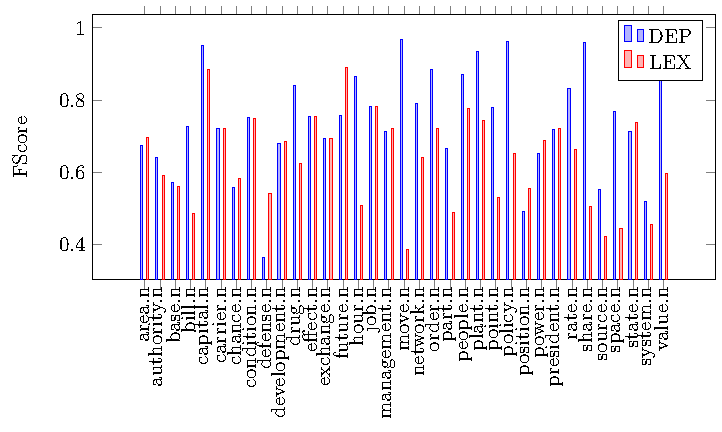
\includegraphics[width=1\linewidth]{images/Chapitre5/tex_img_files/nouns_fs.pdf}
\caption{Unsupervised F-Score results for the nouns of the Semeval 2007 test set}
\label{fig:nouns_fs}
\end{figure}

 \begin{figure}[!htb]
\centering
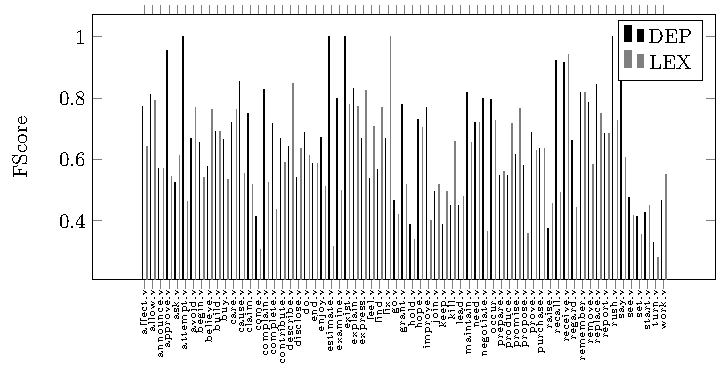
\includegraphics[width=1\linewidth]{images/Chapitre5/tex_img_files/verbs_fs.pdf}
\caption{Unsupervised F-Score results for the verbs of the Semeval 2007 test set}
\label{fig:verbs_fs}
\end{figure}




\paragraph{Semeval-2010}
In Semeval-2010, two unsupervised evaluation metrics are introduced: \textit{V-Measure} and \textit{paired F-Score}. Briefly, the V-Measure assesses the quality of a clustering solution by measuring the degree to which each cluster consists of instances principally belonging to a single gold standard class, or homogeneity; and to completeness, the level with which each gold standard class consists of instances primarily assigned to a single cluster.

The paired F-Score evaluation transforms the clustering problem into a classification one. Two instance pairs sets are generated, the first one coming from the system induced clusters, by including pairs of the instances found in each cluster. The second set of instance pairs is built from the gold standard classes. It contains pairs of the instances found in each class. We can then define \textit{Precision} and \textit{Recall}. Precision is computed as the ratio of the number of common instance pairs between the two sets divided by the total number of pairs in the clustering solution. Recall is the count of common instance pairs between the two sets divided by the total number of pairs in the gold standard. The paired F-Score is the harmonic mean of both quantities.

Concerning the supervised evaluation, it follows explicitly that of Semeval-2007, using recall as the main performance measure. For more details about these measures, we refer the reader to the more comprehensive descriptions found in \cite{Semeval2010,VandeCruys2011,pedersen2010duluth}.


In Table \ref{tab:sem2010_VM} we present our systems compared to the baseline and other methods using during Semeval 2010. V-Measure is a metric well-known for favoring systems producing a higher number of clusters \cite{VandeCruys2011,pedersen2010duluth}. Thus, it is considered not a very reliable metric. We have included it to have a global insight about the performance of our method. We remark that only \textbf{LEX} performed better than both baselines, random assignation of senses (Random) and using the most frequent sense (MFS). Also, we note that we included only the best performing systems, in this case \textit{NMF$_{lib}$} and  \textit{Hermit}. The former  did not participate on the competition but was developed later. We include it henceforth to illustrate how systems variate from one position to another depending the metric used to assess the performance. The latter was the best method on this metric from the task challenge. It is important to notice that other systems exist between Hermit and \textbf{LEX}. They were not included for the sake of clarity.

The second unsupervised measure, Paired F-Score, can be seen in Table \ref{tab:sem2010_FS}. In this case both systems presented performed better than the random baseline. Any system presented was able to beat the MFS baseline. We note that \textbf{DEP} does much better compared to \textbf{LEX} concerning verbs, namely 58\% vs. 28\% F-Score. Still, the results are low considering the best results of the competition, 63\% from Duluth, although again, it generates a number of senses very similar to the MFS baseline. Both our systems induce a considerable amount of clusters while keeping a descent F-Score.

Finally, we in Table \ref{tab:sem2010_SR} we show the supervised Recall results of Semeval-2010. The best performing algorithm shown is NMF$_{lib}$. During the competition, UoY(2010) was the best method. It is a graph-based algorithm which shares the name with the UoY  system presented in Semeval-2007, but it is a different  approach. 

Concerning our systems, in this evaluation they seem to perform the best, or in a comparable level, to the top methods.  We find that in general our systems seem to perform better on the Semeval-2007 dataset. Discovering the reason could shed light into improving the performance on the Semeval-2010 test set. Given the results, it seems like a combination of features (syntactic plus lexical) in  a single algorithm could yield better results. 

As a side note, it is argued that supervised Recall is not a very robust metric as the supervised method within tends to converge towards the most frequent sense. In this regard, several researchers \cite{VandeCruys2011,pedersen2010duluth} have voiced their concerns about the quality of the current WSD/WSI evaluation metrics as well as the need of new, more robust techniques to properly evaluate these systems.

%We evaluate our systems by means of the F-score and a precision-recall curve which provides a deeper analysis of the performance of each system while considering the variation of threshold $th_3$.


% As test set, we employ the data provided for Task 02 of Semeval-2007 \cite{semeval2007task2} which evaluated word sense induction systems. The dataset consists on 100 target words\footnote{We note that for this experiment we worked solely with nouns.} (65 verbs and 35 nouns), each target word having a set of paragraph contexts where it appears. From the available performance assessing techniques, we are  interested in the unsupervised evaluation, which is rated using the F-score produced by the furnished evaluation script. We modify it to obtain also the precision and recall measures. 
 
 
 
% \begin{figure}[]
% \begin{minipage}{0.48\textwidth}
%   \centering
%    \begin{tabular}{ll}
%    \hline
%    \textbf{System} & \textbf{\begin{tabular}[c]{@{}l@{}}Nouns \\ FSc.\end{tabular}} \\ \hline
%    
%    {dep}            & 80.6                                                         \\
%    {lex}              & 79.5                                                           \\ \hline
%    \end{tabular}
%  \caption{Best F-scores obtained for both our methods on Task 02 of Semeval-2007, using lexical (\textit{lex}) and syntactic dependency (\textit{dep}) co-occurrences. }
%   \label{tab:results}
% \end{minipage}
% \hfill
%\begin{minipage}{.48\textwidth}
%  %\centering
%  \pgfplotsset{height=0.9\columnwidth, width=\columnwidth}
%  \begin{tikzpicture}[]
%    \begin{axis}[
%    xmin=0.94,
%    xmax=1,
%%    ymin=0.73,
%%    ymax=0.755,
%    ylabel={Precision},
%    xlabel={Recall}]
%    \addplot[color=red,mark=x] table [x=recall, y=precision]  {data/deps.tsv};
%    \addplot[color=blue,mark=o] table [x=recall, y=precision]  {data/sens.tsv};
%    \end{axis}
%  \end{tikzpicture}
%  \caption{Precision-Recall curve for \textit{lex} and \textit{dep} systems. To improve visibility, we focused the scale on the curves.}
%  \label{fig:prec_recall}
%\end{minipage}%
%
%\end{figure} 

\begin{table}[]
\centering

\begin{tabular}{@{}lrrrr@{}}
\toprule
\textbf{VM (\%)} & \textbf{all} & \textbf{nouns} & \textbf{verbs} & \textbf{\#cl} \\ \midrule
{Hermit} & 16.2 & 16.7 & 15.6 & 10.78 \\
NMF$_{lib}$&11.8&13.5&9.4&4.80\\
\textbf{LEX} & 11.6 & 8.8 & 11.9 & 10.5 \\
Random & 4.4 & 4.2 & 4.6 & 4.00 \\
\textbf{DEP} & 3.5 & 3.9 & 2.8 & 2.75 \\
MFS & 0.0 & 0.0 & 0.0 & 1.00 \\ \bottomrule
\end{tabular}
\caption{Unsupervised V-Measure (VM) on the Semeval 2010 test set}
\label{tab:sem2010_VM}
\end{table}


\begin{table}[]
\centering

\begin{tabular}{@{}lrrrr@{}}
\toprule
\textbf{FS (\%)} & \textbf{all} & \textbf{nouns} & \textbf{verbs} & \textbf{\#cl} \\ \midrule
MFS & 63.5 & 57.0 & 72.4 & 1.00 \\
Duluth-WSI-SVD-Gap & 63.3 & 57.0 & 72.4 & 1.02 \\
\textbf{DEP} & 53.6 & 50.1 & 58.7 & 2.75 \\
NMF$_{lib}$&45.3&42.2&49.8&5.42\\
\textbf{LEX} & 38.4 & 46.7 & 28.5 & 10.5 \\
Random & 31.9 & 30.4 & 34.1 & 4.00 \\ \bottomrule
\end{tabular}
\caption{Unsupervised Paired F-Score (FS) for the Semeval 2010 test set}
\label{tab:sem2010_FS}
\end{table}


\begin{table}[h!]
\centering

\begin{tabular}{@{}lrrr@{}}
\toprule
\textbf{SR (\%)} & \textbf{all} & \textbf{nouns} & \textbf{verbs} \\ \midrule
NMF$_{lib}$&62.6&57.3&70.2\\
UoY(2010) & 62.4 & 59.4 & 66.8 \\

\textbf{LEX} & 59.8 & 55.8 & 67.4 \\
\textbf{DEP} & 59.3 & 53.9 & 67.2 \\
MFS & 58.7 & 53.2 & 66.6 \\
Random & 57.3 & 51.5 & 65.7 \\ \bottomrule

\end{tabular}

\caption{Supervised recall (SR) for Semeval 2010 test set (80\% mapping, 20\% evaluation)}
\label{tab:sem2010_SR}
\end{table}



The F-score of both systems is shown in Figure \ref{tab:results}. Indeed, in our experiment, the dependency based model \textit{dep} preformed better than \textit{lex} using classic lexical co-occurrence. Even more, in Figure \ref{fig:prec_recall} we   appreciate that even while using different threshold values, we achieve, in general, better recall and precision by using syntactic dependencies. It must be noted  that this particular Semeval task was dominated by the most frequent sense with an F-score of 80.7, assigning an average of one sense per target word. Our solutions assign an average of 1.257 and 1.200 for \textit{lex} and \textit{dep} respectively.



\subsection{Discussion and Conclusion}